\documentclass[11pt,a4paper]{article}

\usepackage[utf8]{inputenc}
\usepackage[T1]{fontenc}
\usepackage[spanish,es-tabla,es-nodecimaldot]{babel}
\usepackage{lmodern}
\usepackage{microtype}
\usepackage[margin=2.5cm]{geometry}
\usepackage{amsmath,amssymb}
\usepackage{graphicx}
\usepackage{booktabs}
\usepackage{tabularx}
\usepackage{array}
\usepackage{xcolor}
\usepackage{enumitem}
\usepackage{caption}
\usepackage{float}
\usepackage[hidelinks]{hyperref}

\graphicspath{{../img/}}
\setlist{itemsep=2pt,topsep=4pt}
\captionsetup{font=small,labelfont=bf}
\newcommand{\code}[1]{\texttt{#1}}
\newcommand{\SI}[2]{#1\,#2}  % cantidad con unidad (sin depender de siunitx)

\title{\textbf{Robot de auto-balanceo de dos ruedas con aprendizaje por refuerzo profundo}\\[4pt]
\large Avance del proyecto final --- CC3104 Aprendizaje por Refuerzo}
\author{Christian Echeverría \and Mario Betancourt\\[2pt]
\small Universidad del Valle de Guatemala\\[2pt]
\small Repositorio: \url{https://github.com/Ctribsz/ProyectoFinal-APR}}
\date{2 de noviembre de 2026}

\begin{document}
\maketitle

\begin{abstract}
Se presenta el avance del proyecto que compara cuatro algoritmos de control continuo de Stable-Baselines3 (DDPG, TD3, SAC y PPO) en la tarea de balancear un robot de dos ruedas simulado en MuJoCo, frente a un controlador PID en cascada como línea base. A la fecha están completos el modelo físico, el entorno de \code{gymnasium} con cuatro niveles de dificultad, el controlador PID y un pipeline de entrenamiento común y reproducible. El PID resuelve los niveles 0 a 2 sin caídas, pero falla en 13 de 20 episodios del nivel 3, que agrega ruido de sensores, latencia y física aleatorizada. Una primera prueba de humo confirma que el entorno se puede aprender: SAC y TD3 llegan al retorno máximo en menos de 30\,000 pasos, aunque TD3 depende fuertemente de la semilla. El código, las pruebas y la documentación están en \url{https://github.com/Ctribsz/ProyectoFinal-APR}.
\end{abstract}

\section{Pregunta de investigación}

\begin{quote}
¿Qué algoritmo ofrece el mejor desempeño para el auto-balanceo robusto ante perturbaciones, y qué mecanismos técnicos de cada algoritmo explican ese resultado?
\end{quote}

El proyecto busca evitar que la comparación se reduzca a entrenar cuatro veces con valores por defecto. Para eso usa:
\begin{itemize}
  \item un entorno propio con niveles de dificultad crecientes;
  \item el mismo presupuesto de afinamiento y de pasos para todos los algoritmos, con varias semillas;
  \item diagnósticos internos (sobreestimación de $Q$, entropía, KL, suavidad de las acciones) que expliquen los resultados;
  \item una línea base clásica, para saber si el aprendizaje por refuerzo aporta algo frente al control tradicional.
\end{itemize}

Las hipótesis se escriben antes de los experimentos finales:
\begin{description}[font=\normalfont\bfseries]
  \item[H1] TD3 sobreestima menos $Q$ que DDPG y por eso entrena de forma más estable.
  \item[H2] SAC se recupera mejor de empujones grandes, por la exploración que le da la entropía.
  \item[H3] PPO necesita más pasos de entorno, pero tiene menor varianza entre semillas.
  \item[H4] Los agentes igualan al PID en el nivel 0 y lo superan en los niveles 2 y 3.
\end{description}

\section{Diseño del entorno}

\subsection{Modelo físico}

El robot se modela en MJCF como un chasis rectangular de \SI{1.0}{kg} y \SI{0.30}{m} de alto que pivota sobre dos ruedas coaxiales de \SI{4}{cm} de radio y \SI{0.05}{kg}, separadas \SI{18}{cm}. Cada rueda tiene un motor de hasta \SI{0.3}{N\,m}. La física corre a \SI{500}{Hz} y el control a \SI{100}{Hz}. La fricción rueda--suelo es de 1.5, porque con 1.0 las ruedas patinan a torque máximo.

Los sensores imitan a un robot real: una IMU (cuaternión de orientación, giroscopio con saturación en $\pm$\SI{2000}{°/s} y acelerómetro) y encoders en las ruedas (saturación en $\pm$\SI{100}{rad/s}).

La convención de ejes está verificada con pruebas automáticas: $x$ hacia adelante, $y$ sobre el eje de las ruedas y $z$ hacia arriba. Un pitch $\theta>0$ significa que el robot se inclina hacia adelante, y un torque positivo lo hace avanzar e inclina el chasis hacia atrás.

\subsection{Observación, acción y recompensa}

La observación contiene solo lo que podría medir un robot real, con lo que se deja abierta la posibilidad de llevar la política a hardware. Nunca se usa la posición absoluta ni el estado interno del simulador. Los nueve valores se listan en la tabla~\ref{tab:obs}.

\begin{table}[H]
\centering
\caption{Espacio de observación.}
\label{tab:obs}
\begin{tabular}{@{}cll@{}}
\toprule
Índice & Variable & Fuente equivalente \\
\midrule
0 & Pitch $\theta$ & IMU \\
1--2 & Velocidad de pitch $\dot\theta$ y de giro $\dot\psi$ & Giroscopio \\
3--4 & Velocidad de cada rueda (relativa al chasis) & Encoders \\
5--6 & Comandos $v^*$ y $\dot\psi^*$ & Comando externo \\
7--8 & Acción anterior & Memoria del controlador \\
\bottomrule
\end{tabular}
\end{table}

La acción es un comando normalizado $a\in[-1,1]^2$, uno por motor, que se escala al torque máximo. La velocidad lineal se estima con sensores, $v = R\left(\tfrac{\omega_\text{izq}+\omega_\text{der}}{2} + \dot\theta\right)$. La recompensa por paso es una suma ponderada de componentes, y cada uno se registra por separado en los logs:
\begin{equation}
r_t = w_\text{alive} - w_\theta\,\theta^2 - w_{\dot\theta}\,\dot\theta^2 - w_v (v-v^*)^2 - w_{\dot\psi}(\dot\psi-\dot\psi^*)^2 - w_\text{effort}\lVert a_t\rVert^2 - w_\text{smooth}\lVert a_t-a_{t-1}\rVert^2 .
\end{equation}
El episodio termina si $|\theta|>0.6$\,rad (unos 35°, el robot cayó) y se trunca a los 1000 pasos (\SI{10}{s}).

\subsection{Niveles de dificultad}

Los cuatro niveles (tabla~\ref{tab:niveles}) comparten el mismo espacio de observación. Esto es necesario porque se entrena en un nivel y se evalúa en todos.

\begin{table}[H]
\centering
\caption{Niveles de dificultad del entorno.}
\label{tab:niveles}
\begin{tabularx}{\textwidth}{@{}cX@{}}
\toprule
Nivel & Qué agrega \\
\midrule
0 & Balanceo en reposo. \\
1 & Empujones aleatorios: hasta \SI{8}{N} durante \SI{0.1}{s}, uno cada \SI{2}{s} en promedio, aplicados en la parte alta del chasis hacia adelante o atrás. \\
2 & Comandos de velocidad ($\pm$\SI{0.5}{m/s}) y de giro ($\pm$\SI{1}{rad/s}) que cambian cada 2--\SI{4}{s}. \\
3 & Ruido gaussiano en los sensores, latencia de 0--\SI{20}{ms}, masa $\pm$20\,\%, fricción $\pm$30\,\% y torque $\pm$10\,\%. La recompensa usa las lecturas limpias. \\
\bottomrule
\end{tabularx}
\end{table}

\section{Línea base: PID en cascada}

El controlador clásico tiene dos lazos. El lazo externo convierte el error de velocidad en un pitch objetivo; el interno convierte el error de pitch en torque. Para el giro se suma un término diferencial entre ruedas:
\begin{align}
\theta_\text{ref} &= K_{p,v}\,(v^*-v) + K_{i,v}\!\int (v^*-v)\,dt, \\
u &= K_p\,(\theta-\theta_\text{ref}) + K_d\,\dot\theta, \qquad
a_{\text{izq},\text{der}} = u \mp K_{p,\psi}\,(\dot\psi^*-\dot\psi).
\end{align}
El PID usa solo la observación, igual que los agentes, y expone la misma interfaz \code{predict(obs)} que una política de SB3. Las ganancias se eligieron con una búsqueda en rejilla sobre 20 semillas del nivel 0: $K_p=15$, $K_d=0.4$, $K_{p,v}=K_{i,v}=0.05$ y $K_{p,\psi}=0.2$. El lazo interno es estable en un rango amplio ($K_p$ entre 4 y 20). El lazo externo, en cambio, tiene que ser pequeño: con $K_{p,v}\ge 0.2$ el sistema se vuelve inestable, porque para frenar el robot primero tiene que acelerar las ruedas (comportamiento de fase no mínima).

\begin{table}[H]
\centering
\caption{Desempeño del PID por nivel (20 episodios de \SI{10}{s}; retorno máximo 1000).}
\label{tab:pid}
\begin{tabular}{@{}ccccc@{}}
\toprule
Nivel & Caídas & Retorno medio & RMSE $v$ (m/s) & RMSE $\dot\psi$ (rad/s) \\
\midrule
0 & 0/20 & 999.5 & 0.016 & --- \\
1 & 0/20 & 994.8 & 0.547 & --- \\
2 & 0/20 & 809.7 & 0.600 & 0.134 \\
3 & \textbf{13/20} & $-286.7$ & 0.844 & 2.366 \\
\bottomrule
\end{tabular}
\end{table}

El PID resuelve los niveles 0 a 2 (tabla~\ref{tab:pid}). Con un solo empujón a $t=\SI{2}{s}$, tolera hasta \SI{17.3}{N}, medido por búsqueda binaria. En el nivel 3 falla porque, con una ganancia alta en el ángulo, un ruido de \SI{0.01}{rad} en $\theta$ se traduce en $\pm0.15$ de acción, y la latencia lo desestabiliza. Ese es el escenario donde H4 espera que el aprendizaje por refuerzo lo supere. La figura~\ref{fig:pid} muestra la respuesta ante un empujón.

\begin{figure}[H]
\centering
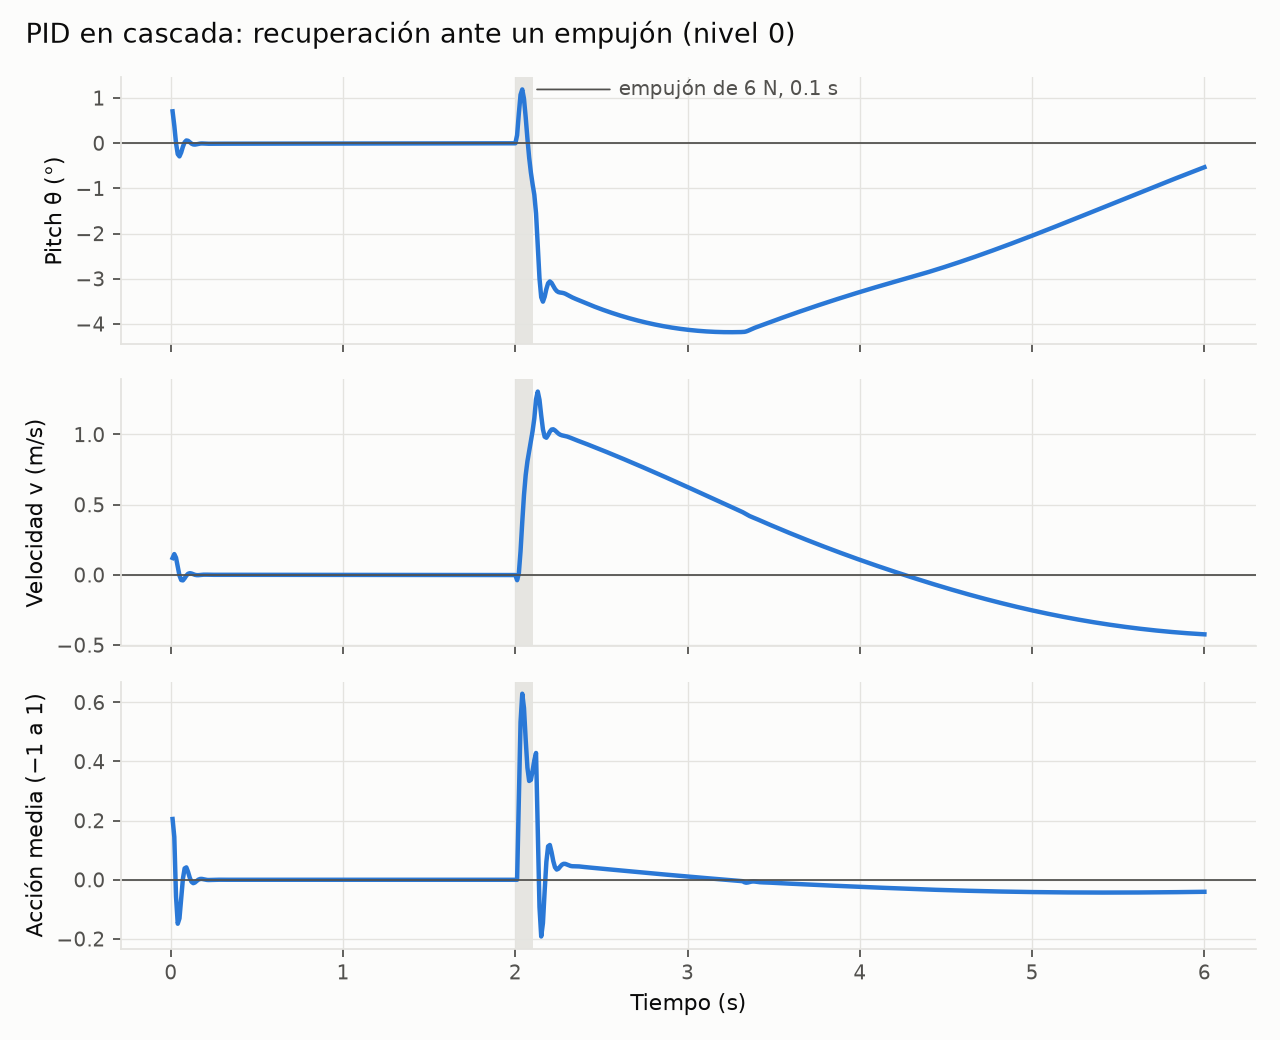
\includegraphics[width=0.72\textwidth]{pid_empujon.png}
\caption{Respuesta del PID a un empujón de \SI{6}{N} en el nivel 0. El lazo de ángulo recupera la vertical en unos \SI{0.2}{s}. El lazo de velocidad es lento por diseño: se inclina $-4$° para frenar y tarda unos \SI{2}{s}.}
\label{fig:pid}
\end{figure}

\section{Pipeline de entrenamiento}

Los cuatro algoritmos pasan por un único script, \code{training/train.py}, y solo cambia el archivo YAML de cada uno. Así ningún algoritmo recibe un tratamiento distinto en la forma de entrenar o evaluar. La arquitectura de red es fija para todos, una MLP $[256,256]$, para que no sea una variable más de la comparación.

Cada corrida guarda todo lo necesario para reproducirla: semilla, configuración completa, versiones de las librerías, commit de git, máquina, duración, evaluaciones periódicas deterministas (con semillas distintas a las de entrenamiento), el modelo y los logs de TensorBoard con cada componente de la recompensa. El repositorio tiene 63 pruebas automáticas que cubren el modelo físico, el entorno, los niveles, el PID y el pipeline; entre otras cosas verifican el determinismo por semilla, los signos físicos y los límites de la observación.

\section{Prueba de humo}

Para confirmar que el entorno se puede aprender, se entrenaron SAC y TD3 con los valores por defecto de SB3 en el nivel 0 durante 100\,000 pasos, con dos semillas y además una corrida con observaciones normalizadas (tabla~\ref{tab:humo} y figura~\ref{fig:humo}).

\begin{table}[H]
\centering
\caption{Prueba de humo en el nivel 0 (100\,000 pasos; retorno máximo 1000).}
\label{tab:humo}
\begin{tabular}{@{}lcccc@{}}
\toprule
Algoritmo & Semilla & Normalizado & Retorno final & Mejor retorno \\
\midrule
SAC & 0 & no & 997 & 998 \\
SAC & 1 & no & 835 & 943 \\
SAC & 0 & sí & 192 & 976 \\
TD3 & 0 & no & 16 & 48 \\
TD3 & 1 & no & \textbf{1000} & 1000 \\
TD3 & 0 & sí & 295 & 588 \\
\bottomrule
\end{tabular}
\end{table}

\begin{figure}[H]
\centering
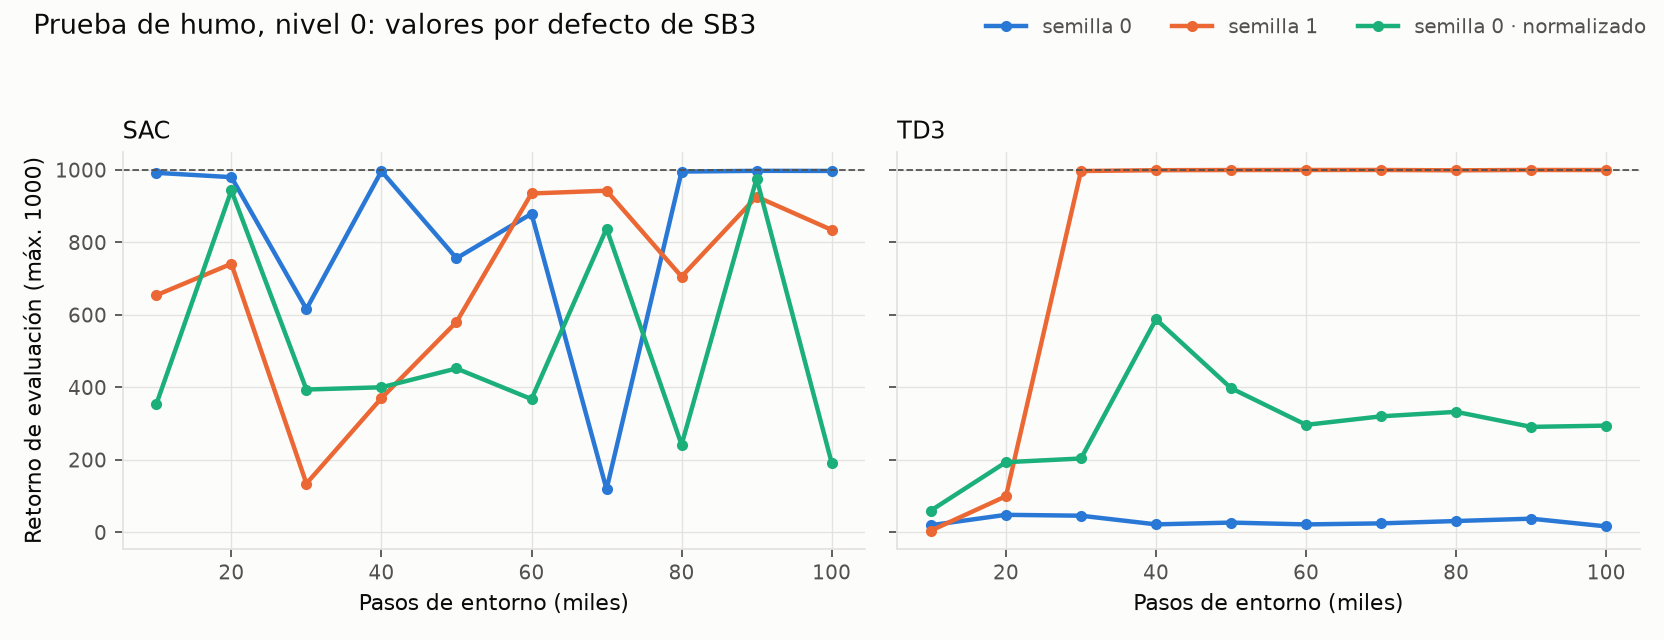
\includegraphics[width=\textwidth]{prueba_humo.png}
\caption{Retorno de evaluación durante la prueba de humo.}
\label{fig:humo}
\end{figure}

\begin{itemize}
  \item \textbf{El entorno se puede aprender.} SAC balancea los \SI{10}{s} completos desde los 10\,000 pasos, y TD3 con la semilla 1 lo logra a los 30\,000 y no vuelve a fallar.
  \item \textbf{SAC aprende rápido pero es inestable}: entre una evaluación y la siguiente oscila entre $\sim$100 y 1000.
  \item \textbf{TD3 depende mucho de la semilla.} Con la semilla 0 nunca aprende en 100\,000 pasos; con la semilla 1 queda perfecto. Esto justifica usar 10 semillas e intervalos de confianza robustos (IQM con bootstrap).
  \item \textbf{Normalizar las observaciones} no da una conclusión clara con una sola semilla; se repetirá con más semillas antes de decidir.
\end{itemize}

Las pruebas de humo de DDPG y PPO están en curso, sobre el mismo pipeline.

\section{Costo computacional}

Se midió la velocidad de entrenamiento en CPU (Ryzen 7 de 8 núcleos, un hilo de PyTorch por proceso). La tabla~\ref{tab:costo} muestra los resultados. En paralelo, la máquina rinde como unos 7 procesos independientes. El protocolo completo (afinamiento con 40 pruebas de Optuna por algoritmo y 10 semillas de un millón de pasos) suma unas 160 horas de CPU, que en paralelo son unas 23 horas de tiempo real. Esto cabe en el cronograma.

\begin{table}[H]
\centering
\caption{Velocidad de entrenamiento medida (nivel 0, MLP $[256,256]$, CPU).}
\label{tab:costo}
\begin{tabular}{@{}lcc@{}}
\toprule
Algoritmo & Pasos/s (1 proceso) & Tiempo para $10^6$ pasos \\
\midrule
SAC & 107 & $\sim$2.6 h \\
TD3 & 171 & $\sim$1.6 h \\
DDPG & 200 & $\sim$1.4 h \\
PPO & 1946 & $\sim$9 min \\
\bottomrule
\end{tabular}
\end{table}

\section{Hallazgos de diseño}

\begin{enumerate}
  \item \textbf{El torque máximo es alto para el tamaño del robot.} Con \SI{0.3}{N\,m} y ruedas de \SI{4}{cm}, la aceleración máxima ($\sim$\SI{13.6}{m/s$^2$}) supera a $g$, y a torque máximo las ruedas se despegan del suelo. Esto puede empujar a los agentes hacia un control brusco, algo que medirá la métrica de suavidad.
  \item \textbf{El punto donde se aplica el empujón importa.} Aplicado en el centro de masa, el robot solo rueda y la prueba no mide el balanceo: el PID toleraba \SI{84}{N}. Por eso se aplica en la parte alta del chasis. Además se restringe a la dirección adelante--atrás, porque un empujón lateral vuelca el robot sobre el eje de las ruedas y ningún controlador puede evitarlo.
  \item \textbf{Empujones demasiado fuertes vuelcan el robot al girar.} Con \SI{15}{N}, el robot sale a $\sim$\SI{2.4}{m/s} y, si recibe un comando de giro, se vuelca de lado. Por eso se fijó $F_\text{max}=\SI{8}{N}$.
\end{enumerate}

\section{Reparto y cronograma}

\begin{itemize}
  \item \textbf{Christian Echeverría:} modelo físico, entorno y niveles, PID, pipeline de entrenamiento y afinamiento, diagnósticos, evaluación, y los algoritmos TD3 y SAC.
  \item \textbf{Mario Betancourt:} DDPG y PPO (configuración, espacio de búsqueda, afinamiento, corridas finales y análisis de sus diagnósticos).
  \item \textbf{Ambos:} análisis estadístico, informe y dictamen.
\end{itemize}

\begin{table}[H]
\centering
\caption{Próximos pasos.}
\begin{tabularx}{\textwidth}{@{}lX@{}}
\toprule
Fecha & Actividad \\
\midrule
3--5 nov & Prueba de humo de DDPG y PPO; decidir el presupuesto de pasos y la normalización de observaciones. \\
6 nov & Afinamiento con Optuna (\code{tune.py}) y callbacks de diagnóstico: sobreestimación de $Q$, entropía y KL. \\
7--8 nov & Afinamiento de los cuatro algoritmos en el nivel 2; evaluación y prueba de empujón. \\
9--10 nov & Diez semillas por algoritmo; experimentos de curvas de aprendizaje, generalización entre niveles, empujón, aleatorización y comparación con el PID. \\
11--13 nov & Análisis estadístico con \code{rliable} (IQM, intervalos bootstrap), contraste de H1--H4 e informe final. \\
\bottomrule
\end{tabularx}
\end{table}

\end{document}
